
%%% -----------------------------------------------------------------------
% Dissertation.tex 2025/11/17 version V1.2
%%% -----------------------------------------------------------------------
% This is the official ieee style template for graduate thesis/dissertation at Towson University
% Modified and refined by Yixin Chen, November, 2025
% Any issues or questions contact Yixin Chen via ychen6@students.towson.edu
% Compile this with pdflatex
% Check latest update via this read only link https://www.overleaf.com/read/gbxnfhvxdthj#202aff
%%% -----------------------------------------------------------------------
%% Importance Notice and Tips:
% This template has already make sure the line spacing, margins and most of the format settings are correct.
% But the student will have to make sure the followings
% 
% ``At least two sentences in each paragraph.''
% 
% Also, try to better arrange your figures/tables. LaTeX does not guarantee this.
% whenever you include a figure/table
% makesure you are adding [htbp] as \begin{figure/table}[htbp]
% this will help with the figures/tables and arrange them at the place in text as precisely as possible
% but you still need to slightly adjust the place where you need to include the figure/table
% make sure your figures/tables do not interrupt the paragraphs
% 
% for the chapter headings and figure/table captions, always capitalize the first character to make sure the format of SmallCap can be applied correctly
% 
% when you need to write quotation marks in LaTeX, use `` as the beginning and '' as the ending. e.g., ``example quotation''
% 
% This is a rare case. If there is a single number or character at the end of a paragraph, use a ~ mark to connect them. e.g., ``xxxxxxxx and here is the last objective~i.''
% in this way, ~ will be rendered as a space and make sure the last character ``i'' will not be isolated in a new line.
%%% -----------------------------------------------------------------------
\documentclass{TUgrad}
\usepackage{pdfpages}
%%% -----------------------------------------------------------------------
%% replace with your title, no need to type in capital, the template will make capital automatically
% use \\ to break the lines and make the title inverse pyramid looking
\thesistitle{
Agentic Environment Synthesis: Evaluating the Efficacy of Model Context Protocol (MCP) in Reducing Hallucinations of Declarative System Configuration.
}
%% replace with your name
\authorname{Luis Dale Gascon}
%% Master's and Audiology students: Change to "thesis",
% Others use "dissertation"
\submissiontype{thesis} 
%% Change to reflect your degree: 
% Master of Arts 
% Master of Science 
% Master of Education
% Doctor of Audiology
% Doctor of Philosophy
\degreename{Master's of Computer Science} 
\departmentname{Department of Computer and Information Sciences}
%% Make sure to delete parentheses and comma. Example: May 2025
% Graduation month must be May, August, or December
\graduationdate{December}
%%% -----------------------------------------------------------------------
%% optional acknowledgments page
% uncomment \useack to activate, or comment to deactivate
\useack
%% optional abbrevations page
% uncomment \useabbr to activate, or comment to deactivate
% \useabbr
%% default without numbering headings
% uncomment \usenumbering to activate, or comment to deactivate
% \usenumbering
%% default without highlight for references and links
% uncomment \hypersetup{hidelinks} to activate, or comment for proofreading
% final submission requires no highlight! make sure you have \hypersetup{hidelinks} activated!
\hypersetup{hidelinks}
%%% -----------------------------------------------------------------------
%% main document begins here, do not change this part
\begin{document}
\beforepreface
\afterpreface
%%% -----------------------------------------------------------------------
%%% -----------------------------------------------------------------------
%%% -----------------------------------------------------------------------
%% your work begins as follows, feel free to add or change the chapters
% -------------------------------------------------------------------------
%% Part 1 - Introduction
\chapter{Introduction}\label{chap:intro}

\section{Required Pages}

\section{Paragraph Styles}

In latex/overleaf, use \textbackslash chapter for chapter headings, use \textbackslash section for level 2 headings, use \textbackslash subsection for level 3 headings, use \textbackslash subsubsection for level 4 headings. Read the inline comments for detailed commands. Do not use other commands for headings!

% here are the commands
% \chapter{}        ----chapter headings
% \section{}        ------level 2 headings
% \subsection{}     --------level 3 headings
% \subsubsection{}  ----------level 4 headings
% note that sometimes you may want to use the heading's format but not count it in the table of contents(TOC), use a * mark
% e.g., \section*{} but be careful, unless you know what will happen, do not use this.
% the commands without a * mark should be enough for your thesis/dissertation

\section{Table of Contents, List of Tables, and List of Figures}

\section{How to use references}

In latex/overleaf, use \textbackslash cite\{\} for reference usage and put your bib text in the reference folder. Here is an example~\cite{EI-CPS-Book}.

% the command to cite the references, here ~ is used for a space's placeholder
% ~\cite{}
% put your paper's bibtext in References/mine.bib and others work in References/ref.bib

And you can also use \textbackslash ref\{\} to refer to a chapter/section/subsection/subsubsection or figures/tables with the label. Here is an example: this is Chapter~\ref{chap:intro}.

% -------------------------------------------------------------------------
%% Part 2 - Literature Review
\chapter{Related Works}\label{chap:litreview}

% use \numbering to activate numbering mode in Dissertation.tex

\section{DevContainers to Standardize Student Development Environments}

\cite{valstarUsingDevContainersStandardize2020}

\section{A Survey of using Large Language Models for Generating Infrastructure as Code}

\cite{srivatsaSurveyUsingLarge} concludes that LLMs lack awareness of current best practices

Lorem  ipsum dolor sit amet, consectetur adipiscing elit. Aliquam ac malesuada leo. Aliquam sit amet eros eleifend, molestie quam eu, scelerisque tortor. Etiam vel diam rutrum, maximus arcu nec, tempus magna. Praesent pretium, mauris eget euismod facilisis, libero lorem laoreet leo, at bibendum arcu massa at dui. Aliquam id felis mi. Vivamus egestas efficitur metus, sed semper libero facilisis in. Cras id scelerisque quam, sit amet dictum tellus.

\subsubsection{IEEE Style Heading Level 4}

Lorem  ipsum dolor sit amet, consectetur adipiscing elit. Aliquam ac malesuada leo. Aliquam sit amet eros eleifend, molestie quam eu, scelerisque tortor. Etiam vel diam rutrum, maximus arcu nec, tempus magna. Praesent pretium, mauris eget euismod facilisis, libero lorem laoreet leo, at bibendum arcu massa at dui. Aliquam id felis mi. Vivamus egestas efficitur metus, sed semper libero facilisis in. Cras id scelerisque quam, sit amet dictum tellus.

% -------------------------------------------------------------------------
%% Part 3 - Main Works
% -----Main work 1
\input{Pages/B-Text/cpt3}
% -------------------------------------------------------------------------
% Part 4 - Conclusion
\chapter{Testing Methodology}\label{chap:testing}

\section{Agent flake synthesis testing}

\subsection{Pass@K}

\section{Comparison between Nix and DevContainer hardware resource usage}


% -------------------------------------------------------------------------
% Examples of some special cases and how to handle with them
% please delete/comment the next input line before final submission
\chapter{Examples of Some Special Cases}\label{chap:examples}

Lorem ipsum dolor sit amet, consectetur adipiscing elit. Aliquam ac malesuada leo. Aliquam sit amet eros eleifend, molestie quam eu, scelerisque tortor. Etiam vel diam rutrum, maximus arcu nec, tempus magna. Praesent pretium, mauris eget euismod facilisis, libero lorem laoreet leo, at bibendum arcu massa at dui. Aliquam id felis mi. Vivamus egestas efficitur metus, sed semper libero facilisis in. Cras id scelerisque quam, sit amet dictum tellus. Integer porttitor laoreet iaculis. In hac habitasse platea dictumst. Nullam justo ante, lacinia in tristique sed, vehicula in purus. Phasellus condimentum dapibus mauris, id molestie tortor. Nullam vel ante nulla. Etiam aliquam varius sem, sit amet luctus massa rhoncus in. Praesent eget ex nec lacus tincidunt facilisis nec id ligula. Quisque sollicitudin, massa vitae laoreet aliquam, tortor lacus condimentum ligula, vitae sodales velit mauris ut magna. Duis eleifend vulputate ultricies.

\begin{figure}[htbp]
    \centering
    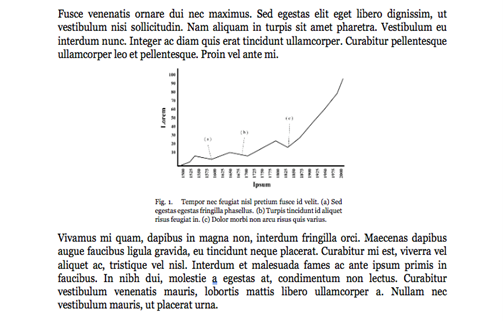
\includegraphics[width=\linewidth]{Figures/Picture1.png}
    \caption{Figure Interrupting The Paragraphs}
    \label{fig:e1}
\end{figure}

\red{This is one of the special cases, we have included the Fig.~\ref{fig:e1} before this paragraph in the code editor. However, the space in the rest of the page is not enough. In this case, the figure will be arranged the first available place in the next page, even interrupting the paragraph afterwards. To solve this, the best way is to manually change the place where the figure is included in the code editor.}

Lorem ipsum dolor sit amet, consectetur adipiscing elit. Aliquam ac malesuada leo. Aliquam sit amet eros eleifend, molestie quam eu, scelerisque tortor. Etiam vel diam rutrum, maximus arcu nec, tempus magna. Praesent pretium, mauris eget euismod facilisis, libero lorem laoreet leo, at bibendum arcu massa at dui. Aliquam id felis mi. Vivamus egestas efficitur metus, sed semper libero facilisis in. Cras id scelerisque quam, sit amet dictum tellus. Integer porttitor laoreet iaculis. In hac habitasse platea dictumst. Nullam justo ante, lacinia in tristique sed, vehicula in purus. Phasellus condimentum dapibus mauris, id molestie tortor. Nullam vel ante nulla. Etiam aliquam varius sem, sit amet luctus massa rhoncus in. Praesent eget ex nec lacus tincidunt facilisis nec id ligula. Quisque sollicitudin, massa vitae laoreet aliquam, tortor lacus condimentum ligula, vitae sodales velit mauris ut magna. Duis eleifend vulputate ultricies. \red{Here we break into a new page to show the same case and how to handle it.}

\newpage

Lorem ipsum dolor sit amet, consectetur adipiscing elit. Aliquam ac malesuada leo. Aliquam sit amet eros eleifend, molestie quam eu, scelerisque tortor. Etiam vel diam rutrum, maximus arcu nec, tempus magna. Praesent pretium, mauris eget euismod facilisis, libero lorem laoreet leo, at bibendum arcu massa at dui. Aliquam id felis mi. Vivamus egestas efficitur metus, sed semper libero facilisis in. Cras id scelerisque quam, sit amet dictum tellus. Integer porttitor laoreet iaculis. In hac habitasse platea dictumst. Nullam justo ante, lacinia in tristique sed, vehicula in purus. Phasellus condimentum dapibus mauris, id molestie tortor. Nullam vel ante nulla. Etiam aliquam varius sem, sit amet luctus massa rhoncus in. Praesent eget ex nec lacus tincidunt facilisis nec id ligula. Quisque sollicitudin, massa vitae laoreet aliquam, tortor lacus condimentum ligula, vitae sodales velit mauris ut magna. Duis eleifend vulputate ultricies. Nullam vel ante nulla. Etiam aliquam varius sem, sit amet luctus massa rhoncus in. Praesent eget ex nec lacus tincidunt facilisis nec id ligula. Quisque sollicitudin, massa vitae laoreet aliquam, tortor lacus condimentum ligula, vitae sodales velit mauris ut magna. Duis eleifend vulputate ultricies.

\blue{This is the example of how to handle this manually. This is the place where Fig.~\ref{fig:e2} is first time referred to. The space in the rest of the page is not enough. We have changed the place where the figure is included. Please check the code editor to see the changes.}

Lorem ipsum dolor sit amet, consectetur adipiscing elit. Aliquam ac malesuada leo. Aliquam sit amet eros eleifend, molestie quam eu, scelerisque tortor. Etiam vel diam rutrum, maximus arcu nec, tempus magna. Praesent pretium, mauris eget euismod facilisis, libero lorem laoreet leo, at bibendum arcu massa at dui. Aliquam id felis mi. Vivamus egestas efficitur metus, sed semper libero facilisis in. Cras id scelerisque quam, sit amet dictum tellus. Integer porttitor laoreet iaculis. In hac habitasse platea dictumst. Nullam justo ante, lacinia in tristique sed, vehicula in purus. Phasellus condimentum dapibus mauris, id molestie tortor. Nullam vel ante nulla. Etiam aliquam varius sem, sit amet luctus massa rhoncus in. Praesent eget ex nec lacus tincidunt facilisis nec id ligula.  \blue{We includ the Fig.~\ref{fig:e2} after this paragraph in the code editor. In this way, there is enough space for the figure between the paragraphs. Including tables should also be in the same way.}

\begin{figure}[htbp]
    \centering
    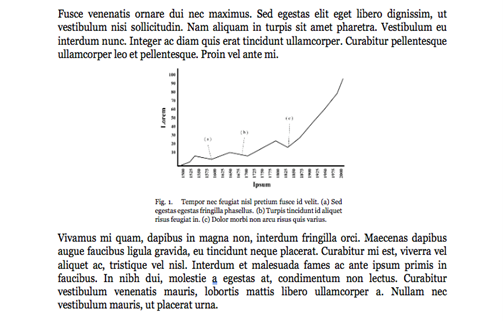
\includegraphics[width=\linewidth]{Figures/Picture1.png}
    \caption{Figure Not Interrupting The Paragraphs}
    \label{fig:e2}
\end{figure}

Lorem ipsum dolor sit amet, consectetur adipiscing elit. Aliquam ac malesuada leo. Aliquam sit amet eros eleifend, molestie quam eu, scelerisque tortor. 

\newpage

Lorem ipsum dolor sit amet, consectetur adipiscing elit. Aliquam ac malesuada leo. Aliquam sit amet eros eleifend, molestie quam eu, scelerisque tortor. Etiam vel Quisque sollicitudin, massa vitae laoreet aliquam, tortor lacus condimentum ligula, vitae sodales velit mauris vitae sodales vut mauris magna. \red{Another special case is, when writing some formula or some explanations, you may write in this way: Lorem ipsum dolor sit amet, consectetur adipiscing adipis  elit. here we denote the second as $s$.}

\blue{You will find that the character $s$ is isolated at the beginning of a new line. This should be avoid. The way to solve this is also included in the very beginning of Dissertation.tex. You can find the solution using \textasciitilde~ in the code editor in the next paragraph.}

Lorem ipsum dolor sit amet, consectetur adipiscing elit. Aliquam ac malesuada leo. Aliquam sit amet eros eleifend, molestie quam eu, scelerisque tortor. Etiam vel Quisque sollicitudin, massa vitae laoreet aliquam, tortor lacus condimentum ligula, vitae sodales velit mauris vitae sodales vut mauris magna. \red{Another special case is, when writing some formula or some explanations, you may write in this way: Lorem ipsum dolor sit amet, consectetur adipiscing adipis  elit. here we denote the second as~$s$.} 

\blue{In this way writing as ``as\textasciitilde$s$'' in the code editor, ``as~$s$'' will be considered to be rendered together to avoid the isolated character in a new line.} It is also recommended always connect your references or refers with a \textasciitilde. Read the code editor for details, e.g. Lorem ipsum~\cite{EI-CPS-Book}, Lorem ipsum Fig.~\ref{fig:e2}.
%%% -----------------------------------------------------------------------
%% Appendix, if no need, comment all this part
\appendix
\input{Pages/C-Supplemental/Appendix-A}
\chapter{Appendix Title Here}\label{apd:b}

[Appendices follow the last page of the text. Each appendix should be labeled, either at the top or on a proceeding blank page, as Appendix A, Appendix B, etc. The sequence of the appendices follows the order in which they were first introduced in the main body of the text. Each appendix needs to be labeled and named in the main body of the text for it to be included in the appendix section.]
%%% -----------------------------------------------------------------------
% References
\bibliographystyle{IEEEtran}
\bibliography{References/ref,References/mine}
%%% -----------------------------------------------------------------------
%% blank page at last, do not change
\clearpage\thispagestyle{empty}\mbox{}\setcounter{page}{0}\clearpage
\end{document}
%%% -----------------------------------------------------------------------
